
\title{fslr: Connecting the FSL Software with R}
\author{by John Muschelli, Elizabeth Sweeney, Martin Lindquist, and Ciprian Crainiceanu}

\maketitle

% No analytic pipeline for processing the data
% Blog post about data
\abstract{
We present the package \CRANpkg{fslr}, a set of R functions that interface with FSL (FMRIB Software Library), a commonly-used open-source software package for processing and analyzing neuroimaging data.  \pkg{fslr} performs operations on \code{nifti} image objects in R using command-line functions from FSL, and returns R objects back to the user.  \pkg{fslr} allows users to develop image processing and analysis pipelines based on FSL functionality while interfacing with the functionality provided by R.  We present an example of the analysis of structural magnetic resonance images, which demonstrates how R users can leverage the functionality of FSL without switching to shell commands.  
}







\renewcommand{\thesubfigure}{\Alph{subfigure}}

%{\scriptsize
%\begin{tabular}{cl}
%\hline
%MRI & Magnetic Resonance Imaging/Image \\
%PD & Proton Density \\
%FLAIR & Fluid-Attenuated Inversion Recovery \\
%MS & Multiple Sclerosis \\ 
%FMRIB & Functional MRI of the Brain Group\\
%MNI & Montreal Neurological Institute \\
%FSL & FMRIB Software Library \\
%FAST & FMRIB's Automated Segmentation Tool \\
%FLIRT & FMRIB's Linear Image Registration Tool \\
%BET & Brain Extraction Tool \\
%FNIRT & FMRIB's Nonlinear Image Registration Tool \\
%\hline
%Glossary of acronyms used
%\end{tabular}
%}

{\scriptsize
\begin{tabular}{cl|cl}
\multicolumn{4}{c}{Glossary of acronyms} \\ \hline
MRI & Magnetic Resonance Imaging/Image & FSL & FMRIB Software Library \\
PD & Proton Density & FAST & FMRIB's Automated Segmentation Tool \\
FLAIR & Fluid-Attenuated Inversion Recovery & FLIRT & FMRIB's Linear Image Registration Tool \\
MS & Multiple Sclerosis & BET & Brain Extraction Tool \\
FMRIB & Functional MRI of the Brain Group & FNIRT & FMRIB's Nonlinear Image Registration Tool \\
MNI & Montreal Neurological Institute \\
\hline
\end{tabular}
}


\section{Introduction}
\label{sec:intro}

FSL (FMRIB Software Library) is a commonly-used software for processing and analyzing neuroimaging data \citep{jenkinson_fsl_2012}.  This software provides open-source command-line tools and a graphical user interface (GUI) for image processing such as image smoothing, brain extraction \citep{smith_fast_2002}, bias-field correction, segmentation \citep{zhang_segmentation_2001}, and registration \citep{jenkinson_global_2001, jenkinson_improved_2002}.    Many of these functions are used extensively in medical imaging pipelines.   According to a recent survey paper by \citet{carp_secret_2012}, 13.9\% of published neuroimaging studies used FSL.

There exist a number of R packages for reading and manipulating image data, including \CRANpkg{AnalyzeFMRI} \citep{bordier_temporal_2011}, \CRANpkg{RNiftyReg} \citep{modat_rniftyreg:_2013}, and \CRANpkg{fmri} \citep{tabelow_statistical_2011} (see the Medical Imaging CRAN task view \url{http://cran.r-project.org/web/views/MedicalImaging.html} for more information).  Although these packages are useful for performing image analysis, much of the fundamental functionality FSL and other imaging software provide is not currently implemented in R.  In particular, this includes algorithms for performing slice-time correction, motion correction, segmentation, bias-field correction, co-registration, and normalization. This lack of functionality is currently hindering R users from performing complete analysis of image data within R.  Instead of re-implementing FSL functions in R, we propose a user-friendly interface between R and FSL that preserves all the functionality of FSL, while retaining the functionality of R.  This will allow
%Moreover, we do not believe they need to be implemented in R directly if readily available.  These implementations aid in using R for neuroimaging analysis and interfacing existing neuroimaging software can help 
R users to implement complete imaging pipelines without necessarily learning software-specific syntax.  

The \CRANpkg{fslr} package relies heavily on the \CRANpkg{oro.nifti} \citep{whitcher_working_2011} package implementation of images (referred to as \code{nifti} objects) that are in the Neuroimaging Informatics Technology Initiative (NIfTI) format as well as other common image formats such as ANALYZE.  \pkg{oro.nifti} also provides useful functions for plotting and manipulating images.  In addition to interfacing FSL and R, \pkg{fslr} expands on the \pkg{oro.nifti} package by adding additional functions for manipulation of \code{nifti} objects.

% , such as \code{cal\_img}, which will reset the \code{cal\_min} and \code{cal\_max} slots on a \code{nifti} object, which are used to determine colors when plotting.

\section{\pkg{fslr} Workflow}
The general workflow for most \pkg{fslr} functions that interface with FSL is as follows:
\begin{enumerate}
\item Filename or \code{nifti} object is passed to \pkg{fslr} function.
\item FSL command is created within \pkg{fslr} function and executed using the \code{system} command.
\item Output is written to disk and/or read into R and returned from the function.
\end{enumerate}

From the user's perspective, the input/output process is all within R.  The advantage of this process is that a user can read in an image, do manipulations of the \code{nifti} object using standard syntax for arrays, and pass this object into the \pkg{fslr} function without using FSL-specific syntax written in a shell language.  Also, one can perform image operations using FSL, perform operations on the \code{nifti} object in R that would be more difficult using FSL, and then perform additional operations using FSL by passing that object to another \pkg{fslr} command.  Thus, users can create complete pipelines for the analysis of imaging data by assessing FSL through \pkg{fslr}. 
%analysis using FSL using only \code{fslr} commands.

\subsection{\pkg{fslr} Setup}
To use \pkg{fslr}, a working installation of FSL is required.  \pkg{fslr} must also have the path of FSL specified.  If using R from a shell environment, and the \code{FSLDIR} environment variable is set (which can be done when installing FSL), \pkg{fslr} will use this as the path to FSL.  If using R through a graphical user interface (GUI) such as RStudio (RStudio, Boston, MA), environmental variables and paths are not explicitly exported.  Therefore, \code{FSLDIR} is not set, and the path to FSL can be specified using \code{options(fsl.path="/path/to/fsl")}. 

\pkg{fslr} also requires an output type for the format of images returned from FSL.  Some \pkg{fslr} functions produce intermediate files that the user may want removed after the command is executed and the extension for the file is required.  If working in a shell environment, \pkg{fslr} will use the environment variable for output type \code{FSLOUTPUTTYPE}.  If working in a GUI, the default is given by \code{NIFTI\_GZ}, which returns compressed NIfTI images, ending in ``.nii.gz''.  This can be changed by setting the \code{fsl.outputtype} option (\code{options(fsl.outputtype="OUTPUTTYPE")}).  See \url{http://fsl.fmrib.ox.ac.uk/fsl/fsl-4.1.9/fsl/formats.html} for a description of FSL output types.

The R code below is all that is needed to load the fslr package, set the path to FSL, and specify the output type for files, respectively.
\begin{knitrout}
\definecolor{shadecolor}{rgb}{0.969, 0.969, 0.969}\color{fgcolor}\begin{kframe}
\begin{alltt}
\hlkwd{library}\hlstd{(fslr)}
\hlkwd{options}\hlstd{(}\hlkwc{fsl.path}\hlstd{=}\hlstr{"/usr/local/fsl"}\hlstd{)}
\hlkwd{options}\hlstd{(}\hlkwc{fsl.outputtype} \hlstd{=} \hlstr{"NIFTI_GZ"}\hlstd{)}
\end{alltt}
\end{kframe}
\end{knitrout}

\subsection{Image Preprocessing with \pkg{fslr}}

We present a complete analysis of structural magnetic resonance imaging (MRI) data performed using \pkg{fslr} and R.  Images were obtained from a patient with multiple sclerosis (MS) at 2 different visits (SWEENEY CITE).  At each visit, the image modalities obtained were T1, T2, fluid-attenuated inversion recovery (FLAIR), and proton density (PD). In this example we will co-register scans within a visit, perform a MRI bias-field correction using FAST (FMRIB's Automated Segmentation Tool) \citep{zhang_segmentation_2001}, co-register scans within visits to the T1 image of that visit, and register T1 images between visits.  Once these operations have been performed, one can take within-modality difference images to see the changes between visits.  We will also register all images to a common stereotaxic template, as this is common in population-based analyses.

\subsection{Bias-Field Correction}

MRI images typically exhibit good contrast between soft tissue classes, but intensity inhomogeneities in the radio frequency (RF) field can cause differences in the ranges of tissue types at different spatial locations.  These inhomogeneities can cause problems with algorithms based on histograms, quantiles, or raw intensities \citep{zhang_segmentation_2001}.  Therefore, corrrection for image homogeneties is a crucial step in many analyses.  FSL implements the bias-field correction from \citet{guillemaud_estimating_1997} in its FAST segmentation pipleine \citep{zhang_segmentation_2001}.  
 






%We have a \code{data.frame} of filenames of the images, and the output filenames for the bias-field inhomogeneity corrected images.  
The \code{fsl\_biascorrect} from \pkg{fslr} will create the corrected images.  We pass in the filename in the \code{file} argument, any additional options, such as \code{-v} for {\bf v}erbose diagnostic outputs, and the {\bf out}put {\bf file}name (\code{outfile}), which is our inhomogeneity-corrected image.



\begin{knitrout}
\definecolor{shadecolor}{rgb}{0.969, 0.969, 0.969}\color{fgcolor}\begin{kframe}
\begin{alltt}
\hlkwd{fsl_biascorrect}\hlstd{(}\hlkwc{file} \hlstd{=} \hlstr{"01-Baseline_T1.nii.gz"}\hlstd{,}
                \hlkwc{outfile}\hlstd{=} \hlstr{"01-Baseline_T1_FSL_BiasCorrect"}\hlstd{,}
                \hlkwc{opts}\hlstd{=} \hlstr{"-v"}\hlstd{)}
\end{alltt}
\end{kframe}
\end{knitrout}




We can observe the difference in voxel values from the baseline T1 image compared to the bias-corrected version in Figure~\ref{fig:bias_correct}.  In panel~\protect\subref*{t1_ortho} we display the T1 image, and in panel~\protect\subref*{bc_t1_ortho} we display the bias-corrected T1 image.  The T1 image is brighter in the middle of the image, while the bias-corrected image is more uniform in white matter (brighter regions).  As this difference may be hard to distinguish visually, we present the scatterplot of these images in Figure~\ref{fig:bias_correct}\protect\subref*{t1_vs_bc_t1}, using the \CRANpkg{ggplot2} package \citep{wickham_ggplot2:_2009}.  Note, both scales are in arbitrary units (a.u.).


\begin{figure}
  \subfloat{
  \label{t1_ortho}
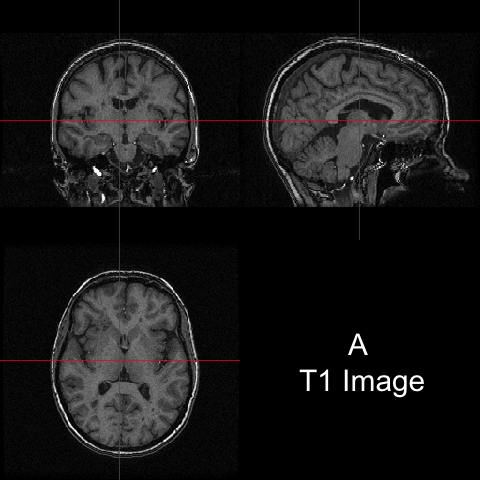
\includegraphics[width = 0.31\textwidth]{figure/T1_Ortho.png}
}
\hfill
  \subfloat{
  \label{bc_t1_ortho}
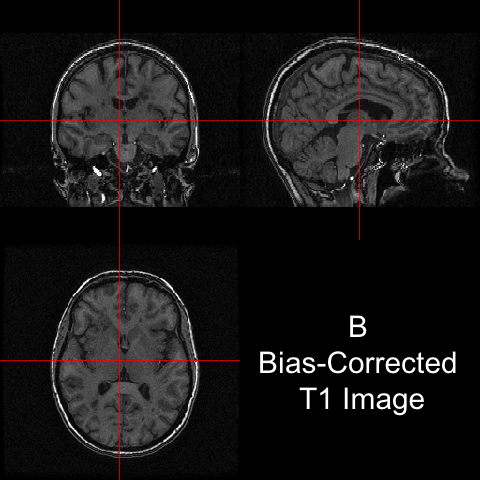
\includegraphics[width = 0.31\textwidth]{figure/BC_T1_Ortho.png} 
}
\hfill
  \subfloat{
  \label{t1_vs_bc_t1}
  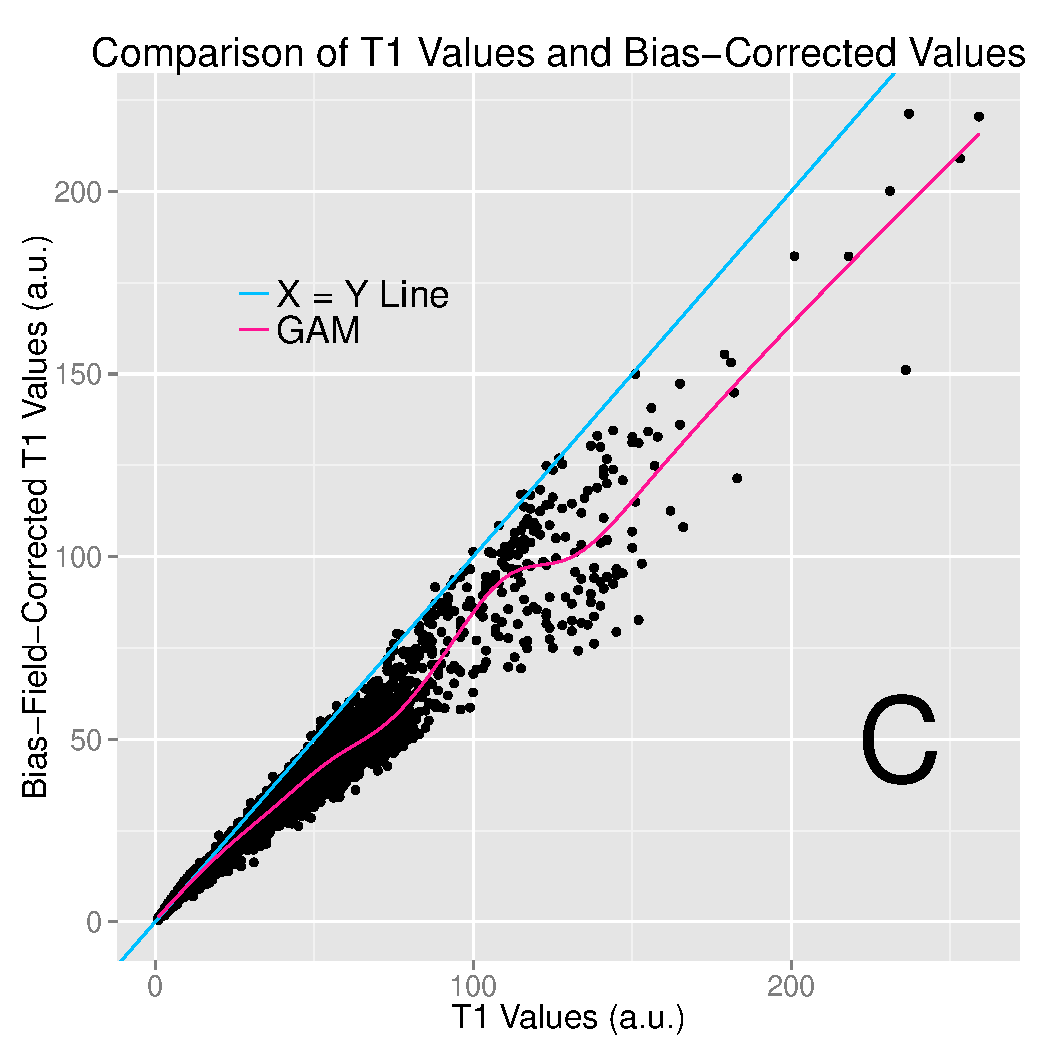
\includegraphics[width = 0.31\textwidth]{figure/plot_bc_data.pdf}
}
\caption{{\bf Results of Inhomogeneity Correction.}  We present the original T1 image~\protect\subref{t1_ortho}, bias-corrected T1 image~\protect\subref{bc_t1_ortho}, and the scatterplot of the sampled values comparing the values from the T1 image and bias-corrected values \protect\subref{t1_vs_bc_t1}.  We see in panel~\protect\subref*{t1_vs_bc_t1} for values in the low range of the data ($< 40$), the T1 values and bias-corrected T1 values, on average, fall along the diagonal (blue line), but values $> 40$ are lower in the bias-corrected T1 values shown by a generalized additive model (GAM) smoother (pink line).  }
\label{fig:bias_correct}
\end{figure}

% Below we subset data where the T1 is not zero, as zero is the background voxel intensity and then subsample the data for visualization.  We also plot the data using \CRANpkg{ggplot2} \citep{wickham_ggplot2:_2009}, shown in figure~\ref{fig:bias_correct}\protect\subref*{t1_vs_bc_t1}.  Note, the scales are in arbitrary units (a.u.).



The blue line in Figure~\ref{fig:bias_correct}\protect\subref*{t1_vs_bc_t1} represents the 45$^{\circ}$ diagonal line, where the original and bias-corrected image intensities are equal, and the pink line represents a generalized additive model (GAM) \citep{hastie_generalized_1990} scatter plot smoother estimate obtained using the \CRANpkg{mgcv} package \citep{wood_fast_2011}.  We see that for values in the low range of the data ($< 40$), the T1 values and bias-corrected T1 values, on average, fall along the diagonal, but values in the higher range are lower in the bias-corrected T1 values.






\section{Within-Visit Co-registration}
In the continuation, all subsequent steps will be performed on the bias-corrected images.  We will first co-register the images within each separate visit to the T1 image from that visit.  This operation overlays the images on one another and allows us to investigate joint distributions of voxel intensities of different image modalities.  This is performed using FMRIB's Linear Image Registration Tool (FLIRT) \citep{jenkinson_global_2001, jenkinson_improved_2002}.  As the images are from the same individual, we may assume that the overall shape of the brain has not changed, but each scan may have undergone a translation and/or rotation in space.  Therefore, we will use a rigid-body transformation, with $6$ degrees of freedom (DOF).  

%We will use another \code{data.frame} with image input and output names, including the T1 image of that visit, the image to be registered, the output transformation matrix and output filename.






The \pkg{fslr} command \code{flirt} will call the FSL command \code{flirt}, taking in the input image (\code{infile}) and the reference image that serves as a template (\code{reffile}).  Any additional options can be passed to the FSL command using the \code{opts} argument.  We will use the defaults (i.e. trilinear interpolation) and the \code{-v} option for diagnostic messages to be printed.  Since we are doing a rigid-body transformation, we set the degrees of freedom (\code{dof}) to 6. Here we present the code for registering the baseline T1 image to the baseline T2 image; we will subsequently repeat this process the T2, FLAIR and PD images, for the baseline and followup scans. 
\begin{knitrout}
\definecolor{shadecolor}{rgb}{0.969, 0.969, 0.969}\color{fgcolor}\begin{kframe}
\begin{alltt}
\hlkwd{flirt}\hlstd{(}\hlkwc{reffile} \hlstd{=} \hlstr{"01-Baseline_T1_FSL_BiasCorrect"}\hlstd{,}
        \hlkwc{infile} \hlstd{=} \hlstr{"01-Baseline_T2_FSL_BiasCorrect"}\hlstd{,}
        \hlkwc{omat} \hlstd{=} \hlstr{"01-Baseline_T2_FSL_BiasCorrect_rigid_to_T1.mat"}\hlstd{,}
        \hlkwc{outfile} \hlstd{=} \hlstr{"01-Baseline_T2_FSL_BiasCorrect_rigid_to_T1"}\hlstd{,}
        \hlkwc{dof} \hlstd{=} \hlnum{6}\hlstd{,} \hlkwc{opts} \hlstd{=} \hlstr{"-v"}\hlstd{)}
\end{alltt}
\end{kframe}
\end{knitrout}



The resulting image transformation will be stored in the file name passed to the \code{omat} ({\bf o}utput {\bf mat}rix) argument.  This matrix can be used to transform other images that were in the same space as the input image to the reference image space.  After co-registration, one could compare images of different modalities at the same voxels, such as T1 versus FLAIR images, which is presented in Figure~\ref{fig:coreg}.  The images are presented at the same cross section for the baseline T1 (Panel~\ref{ft1_ortho}) and FLAIR (Panel~\ref{flair_t1_ortho}) images.  The same brain areas are presented in each modality, indicating adequate registration.  The scatterplot illustrates the joint distribution of intensities for these images; the modalities are in arbitrary units and should not necessarily follow a particular (e.g. linear) relationship.


In the previous example, we present a rigid-body transformation, using the default parameters.  \code{flirt} has options for different cost functions to optimize over, interpolation operators to estimate voxel intensity, and additional degrees of freedom for performing affine transformations.  These options can be passed to the FSL \code{flirt} command using the \code{opts} argument in \code{flirt} in \pkg{fslr}.  

Note that each \pkg{fslr} function has a corresponding help function, which is the \pkg{fslr} command appended with \code{.help()}, which prints out the FSL help page for that function.  For example, users can see which options can be changed in the FSL \code{flirt} command by executing the \code{flirt.help()} function.   Additional non-linear registration techniques are presented in the section~``Registration to the MNI Template''.  







\begin{figure}
  \subfloat{
  \label{ft1_ortho}
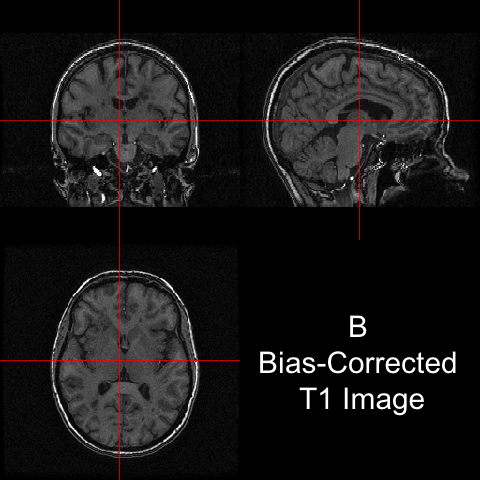
\includegraphics[width = 0.31\textwidth]{figure/BC_T1_Ortho.png}
}
\hfill
  \subfloat{
  \label{flair_t1_ortho}
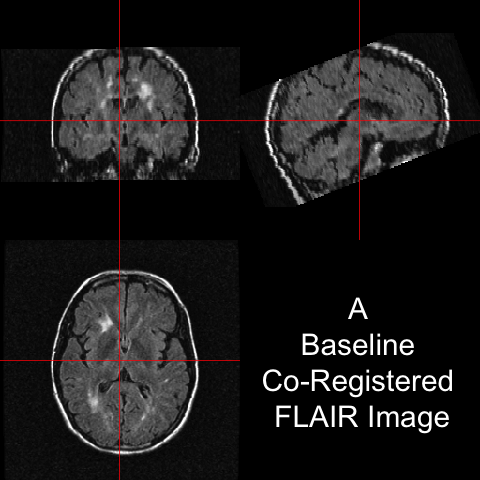
\includegraphics[width = 0.31\textwidth]{figure/FLAIR_Ortho_A_FLIRT.png} 
}
\hfill
  \subfloat{
  \label{t1_vs_flair}
  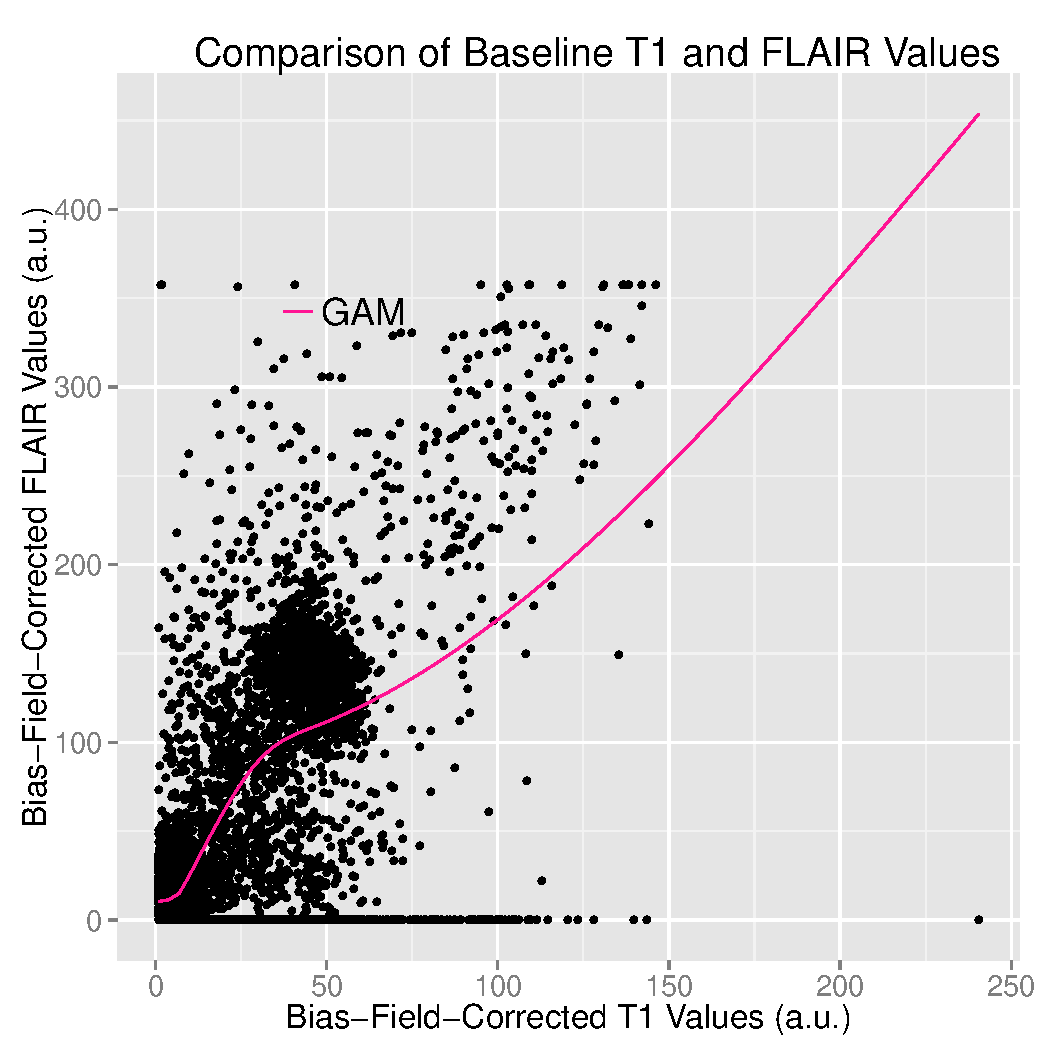
\includegraphics[width = 0.31\textwidth]{figure/plot_flair_t1.pdf}
}
\caption{{\bf Results of within-visit co-registration.}  We present the bias-corrected T1 image~\protect\subref{ft1_ortho}, the co-registered bias-corrected FLAIR image~\protect\subref{flair_t1_ortho}, and the scatterplot of the sampled values comparing the values from the T1 image and bias-corrected values \protect\subref{t1_vs_flair}. Panel~\protect\subref*{t1_vs_flair} displays a scatter plot of the T1 versus Flair data together with a generalized additive model (GAM) smoother (pink line).  }
\label{fig:coreg}
\end{figure}


\section{Between-Visit Co-registration}
Though across-modality comparisons can be achieved by performing within-visit co-registration, across-visit registration is required for assessing within-modality differences between longitudinal scans.   To compute difference images, we co-register followup images to the baseline images within each modality.  Similar to the within-visit co-registration, we use a rigid-body transformation.  We will register the T1 images from baseline and followup, and apply this transformation to the co-registered-to-T1 images from above (see Figure~\ref{fig:reg} for illustration).  

\begin{figure}
\centering
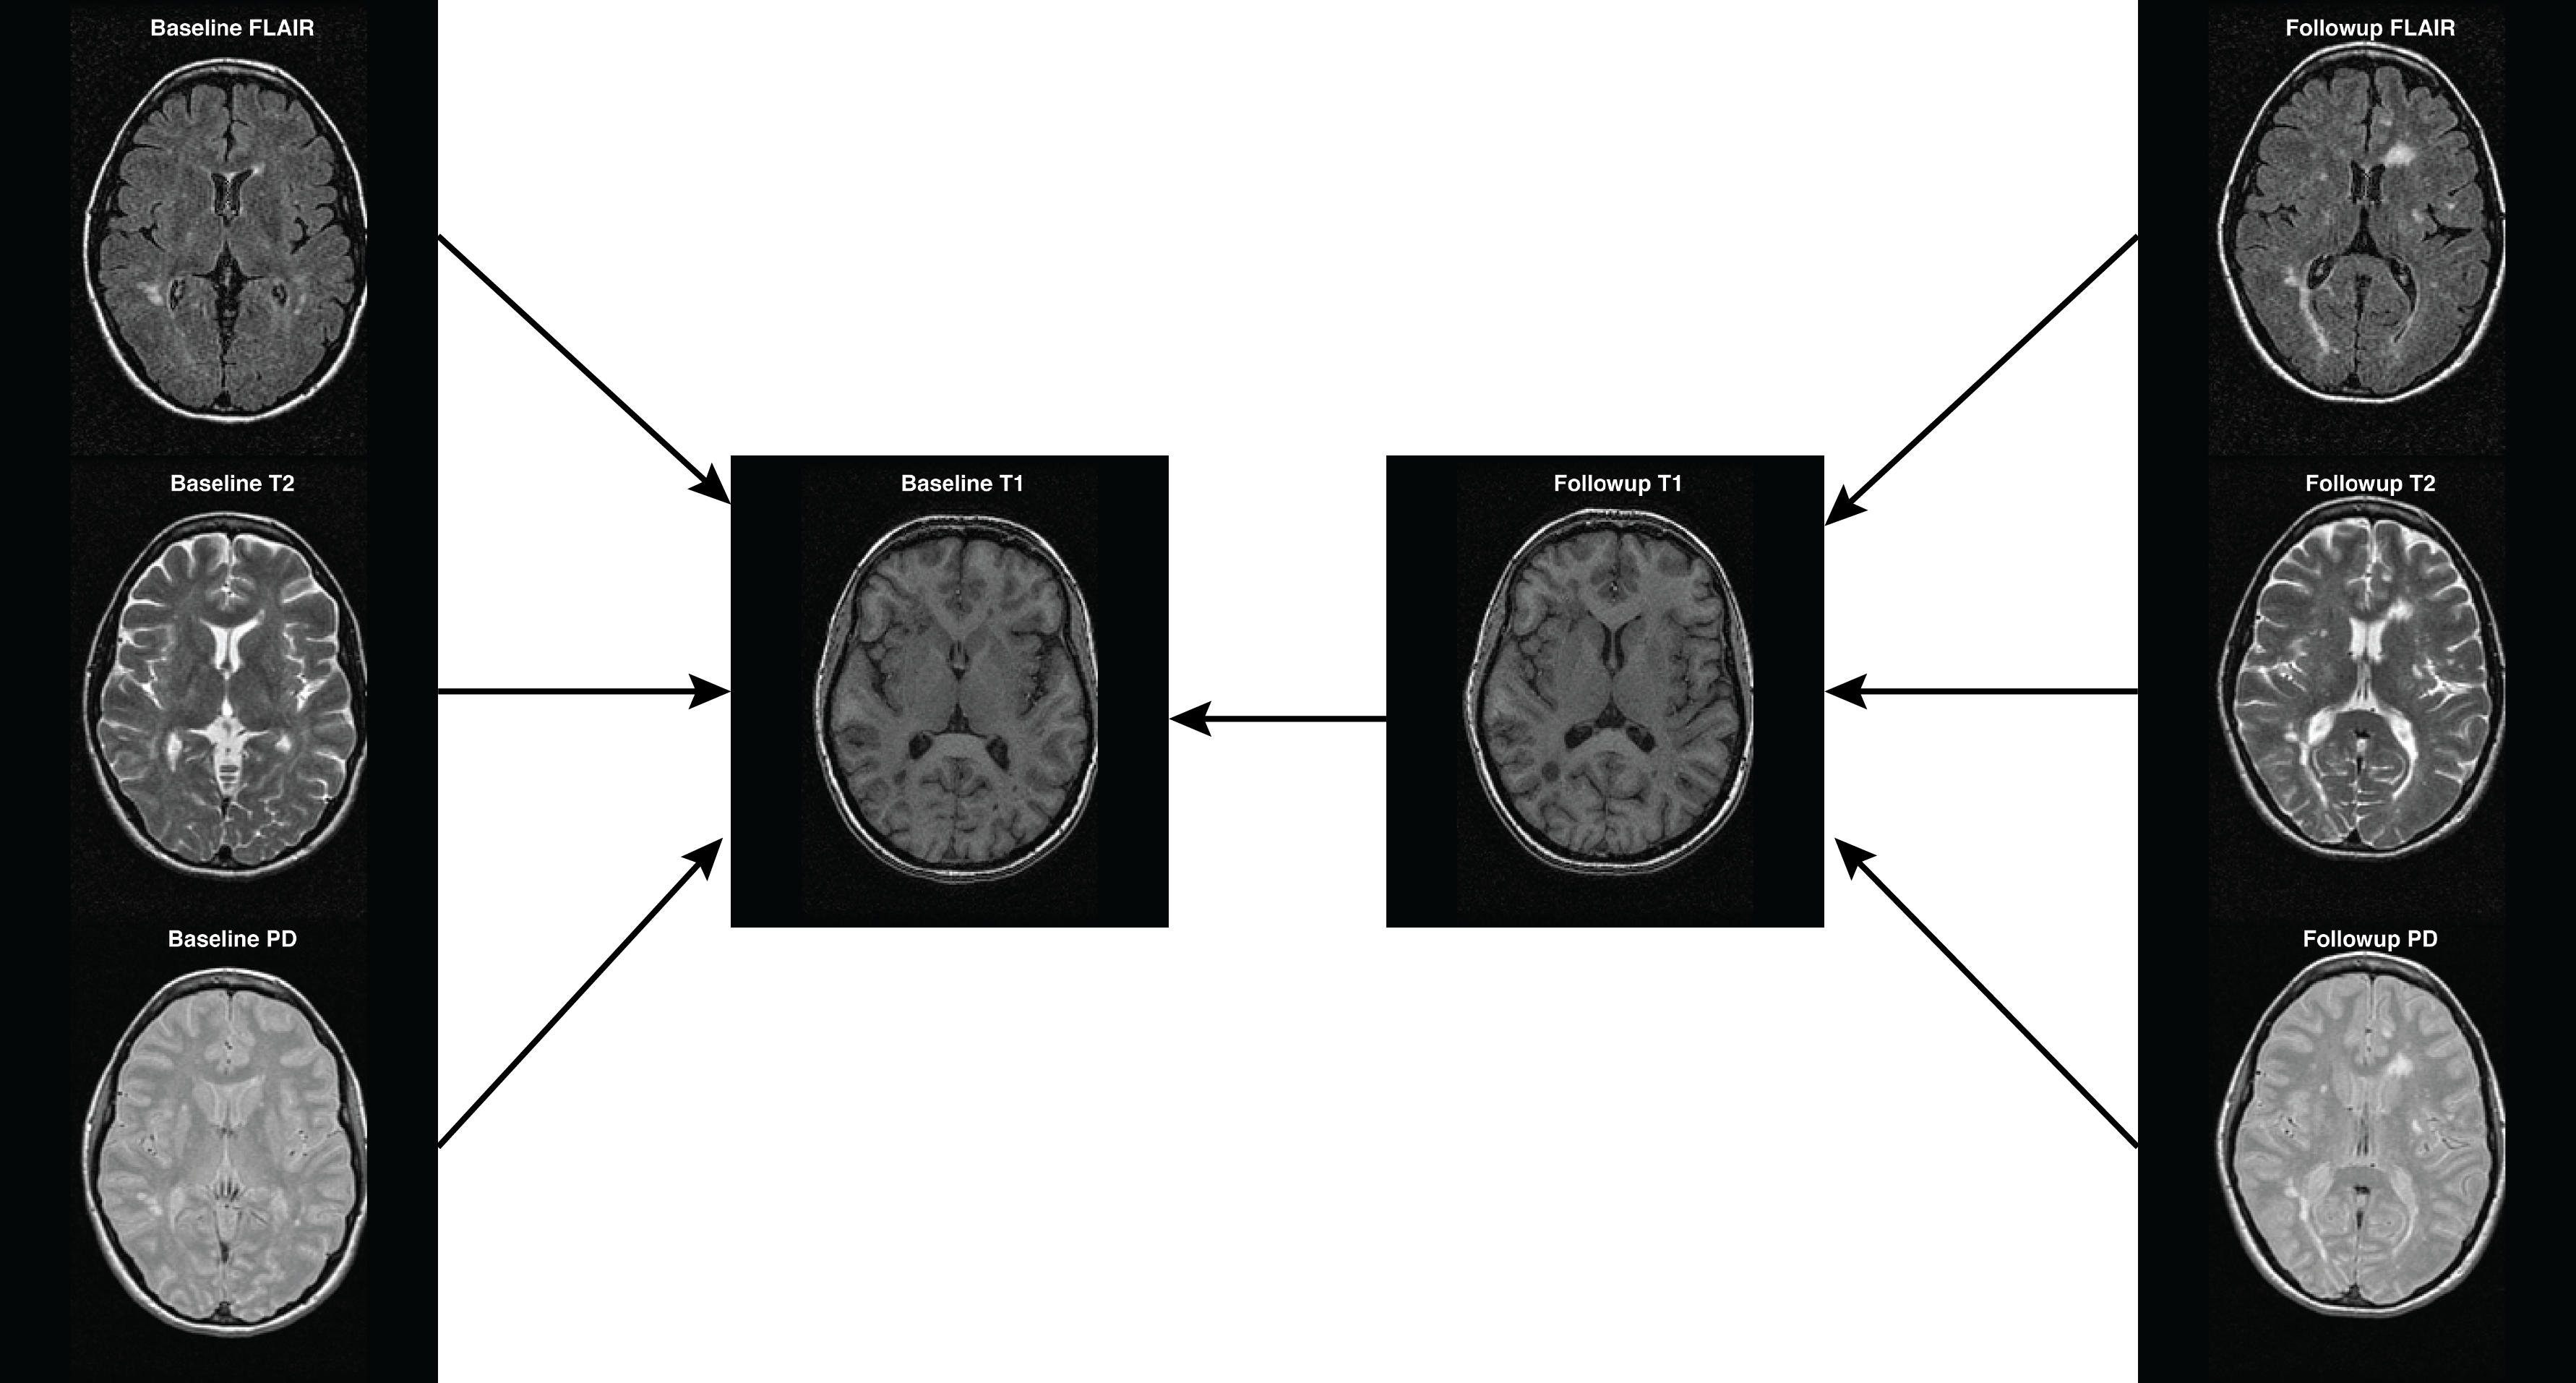
\includegraphics[width = 0.9\textwidth]{Reg_Figure_Option1.png}
\caption{{\bf Between-visit registration process.}  First, we registered all scans within a visit (baseline or followup) to the T1 image.  We then registered the followup T1 image to the baseline T1 image and apply the transformation to the followup T2, FLAIR, and PD images previously co-registered to the followup T1 image. }
\label{fig:reg}
\end{figure}

Though this registration involves two interpolations of the data and may not be optimal for within-modality comparisons, we have already obtained the co-registered-to-T1 images in the section ``Within-Visit Co-registration'' and must perform only one additional registration.  This operation also demonstrates how to apply transformation matrices in \pkg{fslr}.  Here we register the followup T1 image to the baseline T1 image, again using a rigid-body transformation (6 degrees of freedom):

\gobblepars
\begin{knitrout}
\definecolor{shadecolor}{rgb}{0.969, 0.969, 0.969}\color{fgcolor}\begin{kframe}
\begin{alltt}
\hlkwd{flirt}\hlstd{(}\hlkwc{reffile} \hlstd{=} \hlstr{"01-Baseline_T1_FSL_BiasCorrect"}\hlstd{,}
        \hlkwc{infile} \hlstd{=} \hlstr{"01-Followup_T1_FSL_BiasCorrect"}\hlstd{,}
      \hlkwc{omat} \hlstd{=} \hlstr{"01-Followup_T1_FSL_BiasCorrect_rigid_to_BaseT1.mat"}\hlstd{,}
      \hlkwc{dof} \hlstd{=} \hlnum{6}\hlstd{,}
      \hlkwc{outfile} \hlstd{=} \hlstr{"01-Followup_T1_FSL_BiasCorrect_rigid_to_BaseT1"}\hlstd{,}
      \hlkwc{opts} \hlstd{=} \hlstr{'-v'}\hlstd{)}
\end{alltt}
\end{kframe}
\end{knitrout}
\gobblepars


Now, both T1 images are aligned in the space of the baseline T1 image.  We can observe the results in Figure~\ref{fig:flirt}: the bias-corrected baseline T1 image in~\protect\subref*{flirt_base} and the co-registered bias-corrected followup T1 is presented in~\protect\subref*{flirt_fup}.   We observe that the images displayed at the same cross section correspond to the same brain area, indicating a good registration.




\begin{figure}
  \subfloat{
  \label{flirt_base}
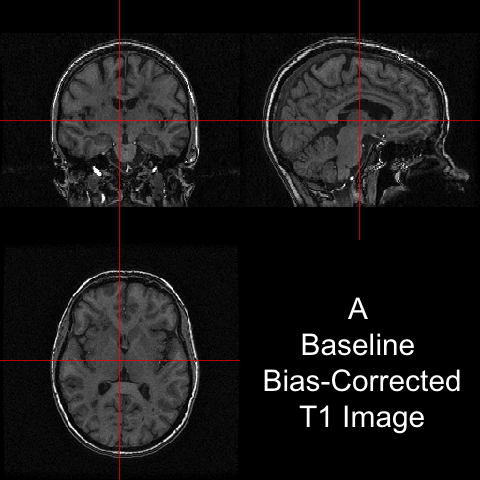
\includegraphics[width = 0.48\textwidth]{figure/BC_T1_Ortho_A.png}
}
\hfill
  \subfloat{
  \label{flirt_fup}
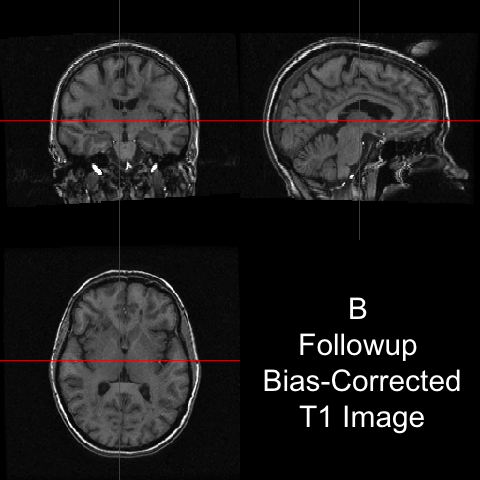
\includegraphics[width = 0.48\textwidth]{figure/FLIRT_Followup_T1.png} 
}
\caption{{\bf Results from FLIRT.} The bias-corrected baseline T1 is presented in~\protect\subref{flirt_base} and the registered bias-corrected followup T1 is presented in~\protect\subref{flirt_fup}, each displayed at the same intersection. We observe that the observed images correspond to the same brain area, indicating a good registration. }
\label{fig:flirt}
\end{figure}


Using the \code{flirt\_apply} function from \pkg{fslr}, we can apply the transformation matrix to the T2, PD, and FLAIR images from the followup visit, previously co-registered to the T1 from followup, to align them to the baseline T1 image space.  The code below aligns the followup T2 image, previously registered to the followup T1 image, to the baseline T1 image:


\begin{knitrout}
\definecolor{shadecolor}{rgb}{0.969, 0.969, 0.969}\color{fgcolor}\begin{kframe}
\begin{alltt}
\hlkwd{flirt_apply}\hlstd{(}\hlkwc{reffile} \hlstd{=} \hlstr{"01-Baseline_T1_FSL_BiasCorrect"}\hlstd{,} \hlcom{# register to this}
            \hlkwc{infile} \hlstd{=} \hlstr{"01-Followup_T2_FSL_BiasCorrect_rigid_to_T1"}\hlstd{,} \hlcom{# reg to Followup T1}
            \hlkwc{initmat} \hlstd{=} \hlstr{"01-Followup_T1_FSL_BiasCorrect_rigid_to_BaseT1.mat"}\hlstd{,} \hlcom{#transform}
            \hlkwc{outfile} \hlstd{=} \hlstr{"01-Followup_T2_FSL_BiasCorrect_rigid_to_BaseT1"} \hlcom{# output file}
            \hlstd{)}
\end{alltt}
\end{kframe}
\end{knitrout}



In Figure~\ref{fig:reg_results}, we display each image after FLIRT has been applied.  Each image is in the baseline T1 image space, displayed at the same cross section.  Each panel shows the same brain areas across modalities, indicating adequate registration.  We see that some areas of the brain are cropped from the field of view, which may be problematic if relevant brain areas are removed.  We have registered all images with the skull and extracranial tissue included.  A better process may be performing registration on brain tissues only, in which case we must perform brain extraction.

\begin{figure}
  \subfloat{
  \label{reg_t1_ortho}
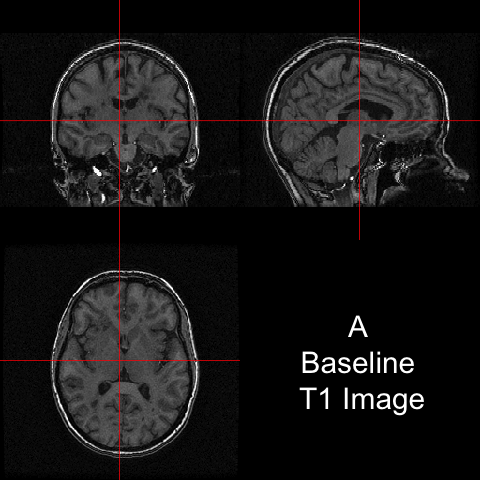
\includegraphics[width = 0.245\textwidth]{figure/BC_T1_Ortho_A_FLIRT.png}
} \hspace*{-0.9em}
\hfill
  \subfloat{
  \label{reg_t2_ortho}
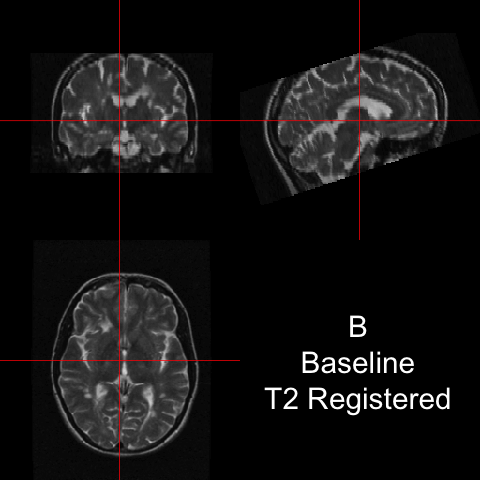
\includegraphics[width = 0.245\textwidth]{figure/01-Baseline_T2_FSL_BiasCorrect_rigid_to_T1.png} \hspace*{-0.9em}
}
\hfill
  \subfloat{
  \label{reg_flair_ortho}
  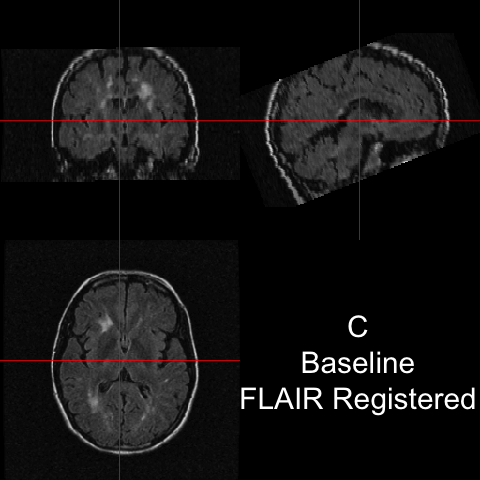
\includegraphics[width = 0.245\textwidth]{figure/01-Baseline_FLAIR_FSL_BiasCorrect_rigid_to_T1.png}\hspace*{-0.9em}
}
\hfill
  \subfloat{
  \label{reg_pd_ortho}
  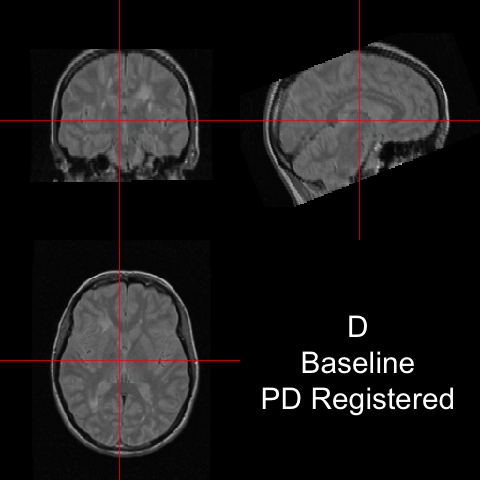
\includegraphics[width = 0.245\textwidth]{figure/01-Baseline_PD_FSL_BiasCorrect_rigid_to_T1.png}
} \hspace*{-0.9em}
\newline
  \subfloat{
  \label{reg_t1_ortho_fup}
  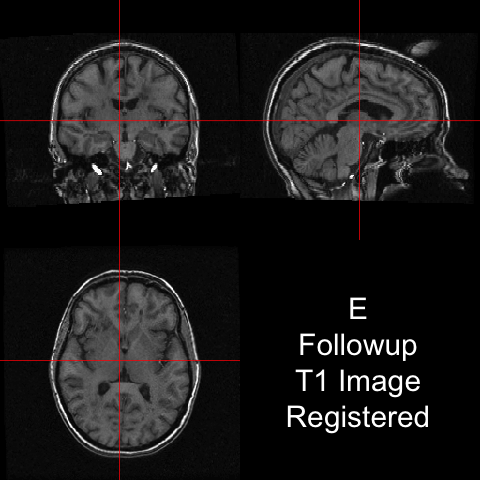
\includegraphics[width = 0.245\textwidth]{figure/E_FLIRT_Followup_T1.png} 
} \hspace*{-0.9em}
\hfill
  \subfloat{
  \label{reg_t2_ortho_fup}
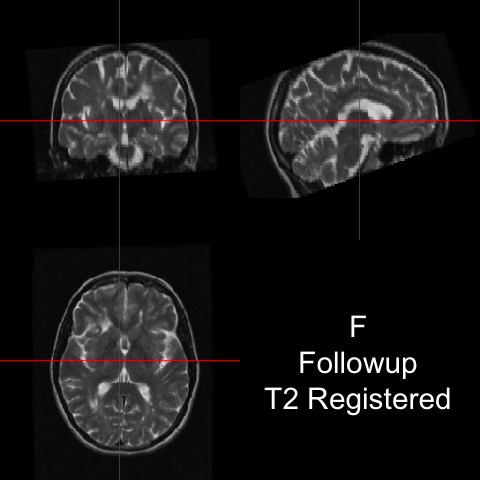
\includegraphics[width = 0.245\textwidth]{figure/01-Followup_T2_FSL_BiasCorrect_rigid_to_BaseT1.png} \hspace*{-0.9em}
}
\hfill
  \subfloat{
  \label{reg_flair_ortho_fup}
  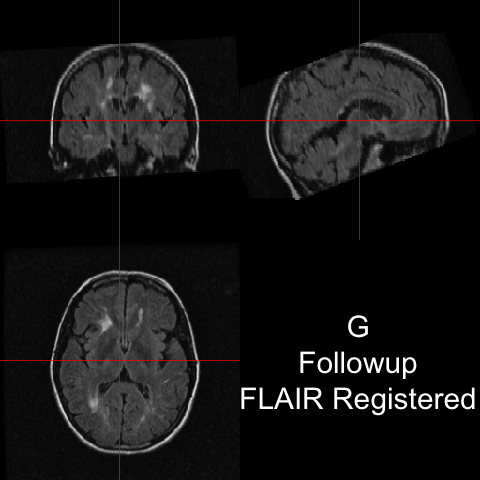
\includegraphics[width = 0.245\textwidth]{figure/01-Followup_FLAIR_FSL_BiasCorrect_rigid_to_BaseT1.png} \hspace*{-0.9em}
}
\hfill
  \subfloat{
  \label{reg_pd_ortho_fup}
  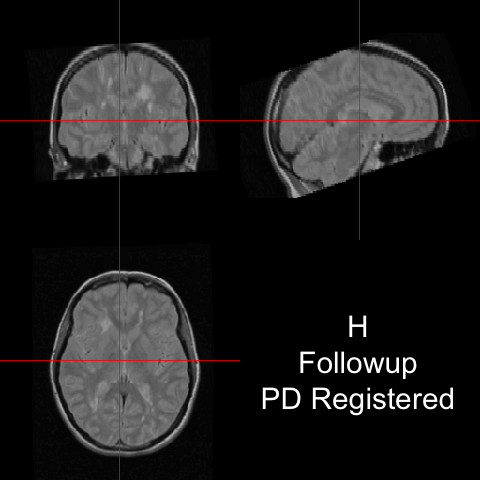
\includegraphics[width = 0.245\textwidth]{figure/01-Followup_PD_FSL_BiasCorrect_rigid_to_BaseT1.png} \hspace*{-0.9em}
}
\caption{{\bf Between-visit registration results.} The complete set of acquired images, first co-registered within visit to the T1 image of that visit, then registered to the baseline T1 image using the followup T1 to baseline T1 transformation matrix.  All registrations performed rigid-body transformations.}
\label{fig:reg_results}
\end{figure}



\section{Brain Extraction}
The process of extracting brain tissue from the acquired image, referred to as brain extraction or skull stripping, is a crucial step in many analyses.  We will perform brain extraction using FSL's brain extraction tool (BET) \citep{smith_fast_2002, jenkinson_bet2:_2005} using parameters recommended by \citet{popescu_optimizing_2012}, which were derived from patients with MS.  No other published R package has brain extraction functionality for brain imaging.  
 


\begin{knitrout}
\definecolor{shadecolor}{rgb}{0.969, 0.969, 0.969}\color{fgcolor}\begin{kframe}
\begin{alltt}
\hlkwd{fslbet}\hlstd{(}\hlkwc{infile} \hlstd{=}  \hlstr{'01-Baseline_T1'}\hlstd{,}
       \hlkwc{outfile} \hlstd{=} \hlstr{"01-Baseline_T1_FSL_BiasCorrect_Brain"}\hlstd{,}
       \hlkwc{opts} \hlstd{=} \hlstr{"-B -f 0.1 -v"}\hlstd{,}  \hlcom{# from Popescu et al.}
       \hlkwc{betcmd} \hlstd{=} \hlstr{"bet"}\hlstd{,}
       \hlkwc{intern}\hlstd{=}\hlnum{FALSE}\hlstd{)}
\end{alltt}
\end{kframe}
\end{knitrout}


We ran BET on the non-corrected T1 image as the \code{-B} option does inhomogeneity correction from FAST as part of the procedure.  The option \code{-f 0.1} denotes the fractional intensity (FI) parameter in BET: it varies between $0$ and $1$ and determines the location of the edge of the segmented brain image; smaller values correspond to larger brain masks. In Figure~\ref{fig:bet}, the bias-corrected T1 image is shown with the brain mask overlaid in red (panel~\protect\subref*{bet_mask}) and the resulting masked brain (panel~\protect\subref*{bet_brain}).  We see that the brain extraction performed well, not including any areas of the skull or the neck while not discarding brain tissue.  Towards the back of the brain, some areas of the subarachnoid space remain, which may be unacceptable for certain analyses, such as estimation of the volume of brain tissue.



\begin{figure}
  \subfloat{
  \label{bet_mask}
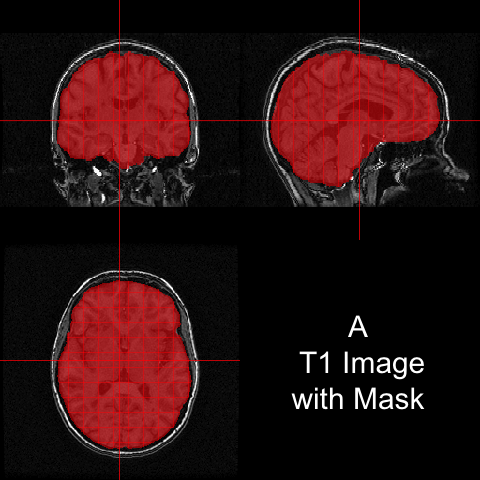
\includegraphics[width = 0.48\textwidth]{figure/plot_bet_mask.png}
}
\hfill
  \subfloat{
  \label{bet_brain}
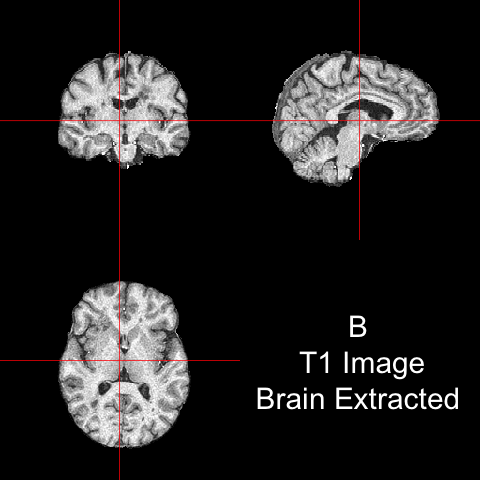
\includegraphics[width = 0.48\textwidth]{figure/plot_bet_brain.png} 
}
\caption{{\bf Results from BET.} In~\protect\subref{bet_mask}, we show the bias-corrected T1 image is presented with the mask from BET overlaid in red.  In~\protect\subref{bet_brain}, we display the extracted brain.  We see that the brain extraction performed well, not including any areas of the skull or the neck while not discarding large areas of the brain.}
\label{fig:bet}
\end{figure}

Note that \code{fslbet} writes both a file containing the brain-extracted image and another image containing the binary brain mask.  As all other images are registered to the baseline T1 space, we can use this mask to extract the brain from other images, such as the baseline T2 image, using the \pkg{fslr} function \code{fslmask}.

\begin{knitrout}
\definecolor{shadecolor}{rgb}{0.969, 0.969, 0.969}\color{fgcolor}\begin{kframe}
\begin{alltt}
\hlkwd{fslmask}\hlstd{(}\hlkwc{file}\hlstd{=}\hlstr{"01-Baseline_T2_FSL_BiasCorrect_rigid_to_T1"}\hlstd{,}
        \hlkwc{mask} \hlstd{=} \hlstr{"01-Baseline_T1_FSL_BiasCorrect_Brain_Mask"}\hlstd{,}
        \hlkwc{outfile} \hlstd{=} \hlstr{"01-Baseline_T2_FSL_BiasCorrect_rigid_to_T1_Brain"}\hlstd{)}
\end{alltt}
\end{kframe}
\end{knitrout}
\gobblepars


We now have all images in the same sterotaxic space with the brain extracted.  

\section{Registration to the MNI Template}
In many studies, information is aggregated across a population of images from different participants.  For the information to have the same interpretation spatially across participants, images from all participants need to be aligned in the same stereotaxic space (``template'' space), requiring registration to a standard template image.  A frequently used set of templates are provided by MNI (Montreal Neurological Institute). We have registered the baseline T1 image to the MNI T1 template \citep{hutchison_symmetric_2006}, included with FSL.  As an individual's brain does not necessarily have the same size as the template, it is not appropriate to use rigid-body transformations.  Instead, non-linear transformations are needed.


We will first register the baseline T1 image to the T1 template using an affine registration, which can perform scaling and shearing operations in addition to translation and rotation.  Although an affine transformation has more degrees of freedom than a rigid transformation, it may not be sufficient for analysis.  We will then use FNIRT (FMRIB's Nonlinear Image Registration Tool) to achieve better overlap of local brain structures \citep{jenkinson_fsl_2012, andersson_non-linear_2007}.  As we are concerned with good overlap only in brain structures, and not in areas such as the skull, we will register the brain-extracted brain images to the brain-only template.  The \pkg{fslr} function \code{fnirt\_with\_affine} will register using \code{flirt} with an affine transformation and then non-linearly register this image to the template using \code{fnirt}.


\gobblepars
\begin{knitrout}
\definecolor{shadecolor}{rgb}{0.969, 0.969, 0.969}\color{fgcolor}\begin{kframe}
\begin{alltt}
\hlkwd{fnirt_with_affine}\hlstd{(}\hlkwc{infile} \hlstd{=} \hlstr{"01-Baseline_T1_FSL_BiasCorrect_Brain"}\hlstd{,}
                  \hlkwc{reffile} \hlstd{=} \hlkwd{file.path}\hlstd{(}\hlkwd{fsldir}\hlstd{(),} \hlstr{"data"}\hlstd{,} \hlstr{"standard"}\hlstd{,} \hlstr{"MNI152_T1_1mm_brain"}\hlstd{),}
                  \hlkwc{flirt.omat} \hlstd{=} \hlstr{"01-Baseline_T1_FSL_BiasCorrect_Brain_affine_toMNI.mat"}\hlstd{,}
                  \hlkwc{flirt.outfile} \hlstd{=} \hlstr{"01-Baseline_T1_FSL_BiasCorrect_Brain_affine_toMNI"}\hlstd{,}
                  \hlkwc{outfile} \hlstd{=} \hlstr{"01-Baseline_T1_FSL_BiasCorrect_Brain_toMNI"}\hlstd{)}
\end{alltt}
\end{kframe}
\end{knitrout}
\gobblepars

\gobblepars

 
The results of the registration can be seen in Figure~\ref{fig:fnirt_slice}.  Each panel represents a different axial slice ($z =$ 25, 45, 92, or 137) in the template space of the template image (\protect\subref*{mni_ortho_25}, \protect\subref*{mni_ortho_45}, \protect\subref*{mni_ortho_92}, \protect\subref*{mni_ortho_137}) or the registered T1 image (\protect\subref*{t1_warp_25}, \protect\subref*{t1_warp_45}, \protect\subref*{t1_warp_92}, \protect\subref*{t1_warp_137}).  Each slice shows the registered T1 image has similar brain structure represented in the same area as the template image, indicating good registration.


% \begin{figure}
%   \subfloat{
%   \label{mni_ortho}
% 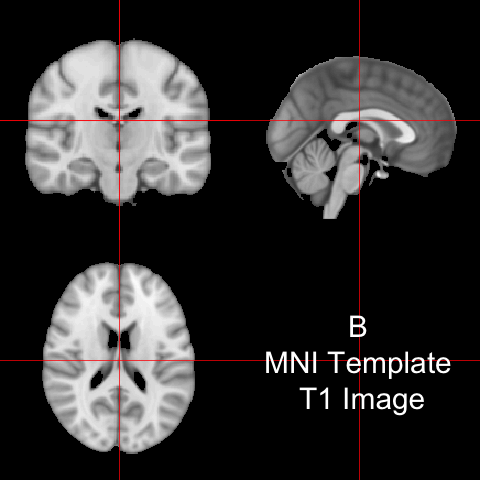
\includegraphics[width = 0.48\textwidth]{figure/MNI_Ortho.png} 
% }
% \hfill
%   \subfloat{
%   \label{t1_warp}
% 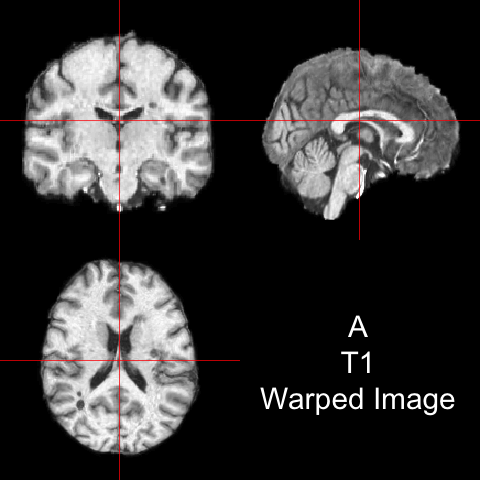
\includegraphics[width = 0.48\textwidth]{figure/T1_MNI_Warp.png}
% }
% \caption{{\bf Results from FNIRT.} In~\protect\subref{mni_ortho}, we display the MNI template image.  In~\protect\subref{t1_warp} we display the registered-to-template, brain-extracted T1 image.  We note that areas of the brain coincide between the template and registered image.}
% \label{fig:fnirt_ortho}
% \end{figure}


\begin{figure}
  \subfloat{
  \label{mni_ortho_25}
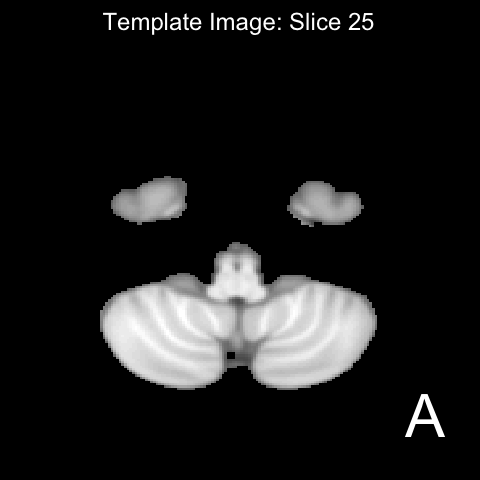
\includegraphics[width = 0.245\textwidth]{figure/MNI_Warp_Slice_25.png} 
} \hspace*{-0.9em}
  \subfloat{
  \label{t1_warp_25}
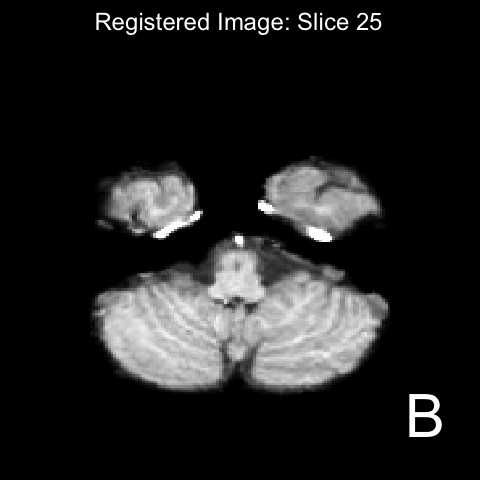
\includegraphics[width = 0.245\textwidth]{figure/T1_MNI_Ortho_Slice_25.png}
} \hspace*{-0.9em}
  \subfloat{
  \label{mni_ortho_45}
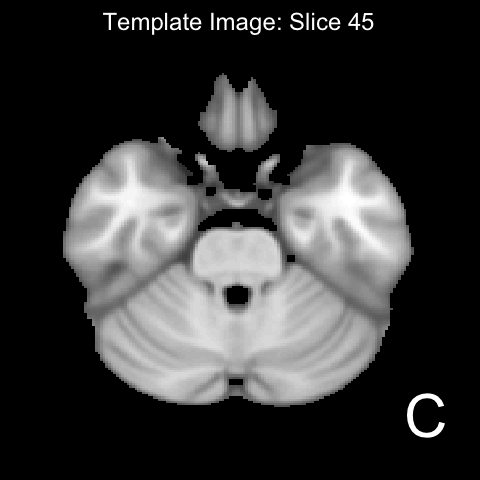
\includegraphics[width = 0.245\textwidth]{figure/MNI_Warp_Slice_45.png} 
} \hspace*{-0.9em}
  \subfloat{
  \label{t1_warp_45}
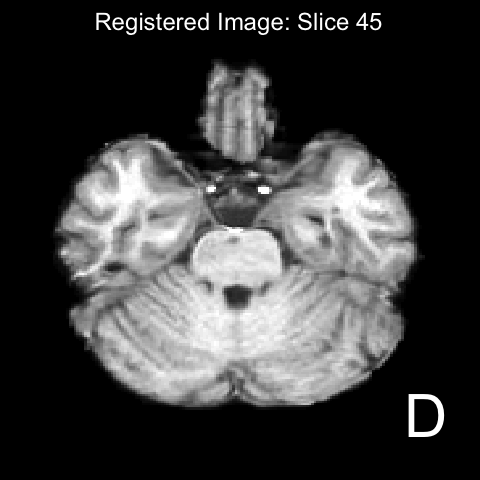
\includegraphics[width = 0.245\textwidth]{figure/T1_MNI_Ortho_Slice_45.png}
}\hspace*{-0.9em}
\newline
  \subfloat{
  \label{mni_ortho_92}
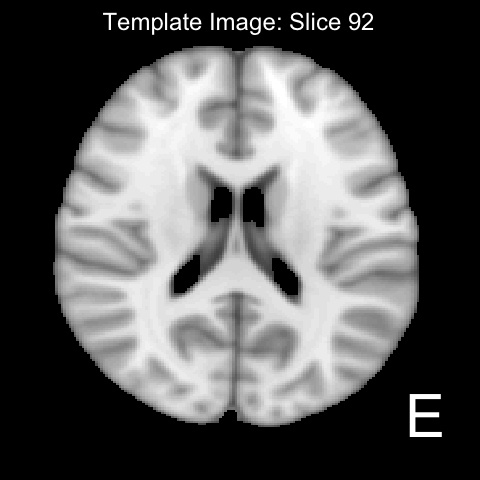
\includegraphics[width = 0.245\textwidth]{figure/MNI_Warp_Slice_92.png} 
} \hspace*{-0.9em}
  \subfloat{
  \label{t1_warp_92}
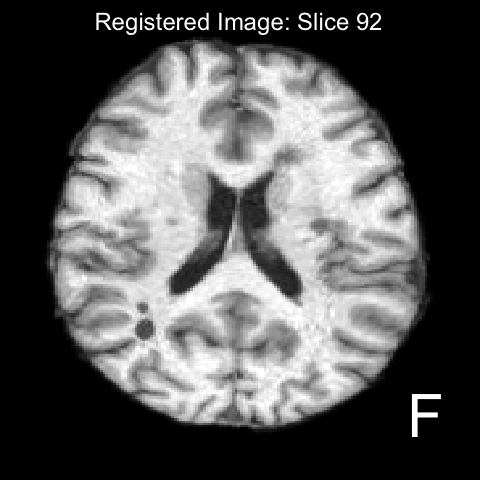
\includegraphics[width = 0.245\textwidth]{figure/T1_MNI_Ortho_Slice_92.png}
} \hspace*{-0.9em}
  \subfloat{
  \label{mni_ortho_137}
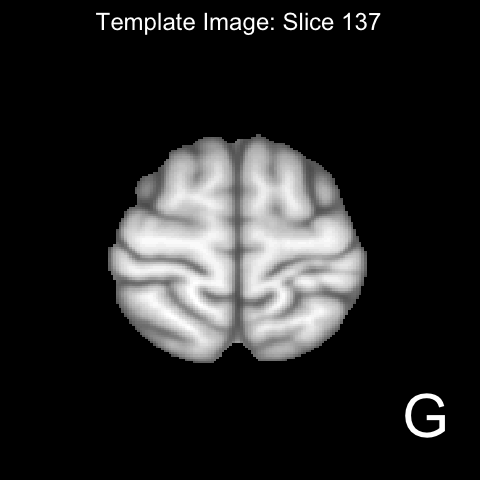
\includegraphics[width = 0.245\textwidth]{figure/MNI_Warp_Slice_137.png} 
} \hspace*{-0.9em}
  \subfloat{
  \label{t1_warp_137}
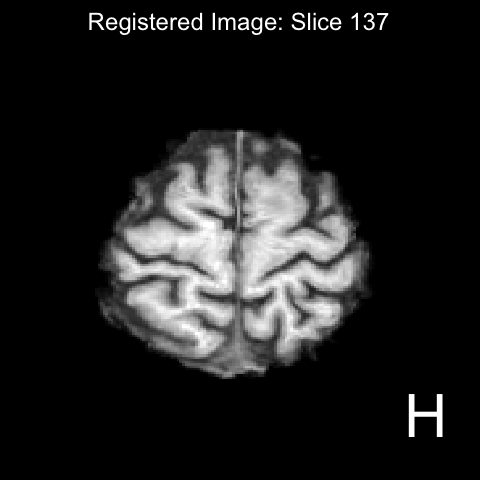
\includegraphics[width = 0.245\textwidth]{figure/T1_MNI_Ortho_Slice_137.png}
}\hspace*{-0.9em}
\caption{{\bf Results from FNIRT.} We present different axial slices of the template (\protect\subref*{mni_ortho_25}, \protect\subref*{mni_ortho_45}, \protect\subref*{mni_ortho_92}, \protect\subref*{mni_ortho_137}) and the registered T1 image (\protect\subref*{t1_warp_25}, \protect\subref*{t1_warp_45}, \protect\subref*{t1_warp_92}, \protect\subref*{t1_warp_137}).  The slices represented are 25 (\protect\subref*{mni_ortho_25}, \protect\subref*{t1_warp_25}), 45 (\protect\subref*{mni_ortho_45}, \protect\subref*{t1_warp_45}), 92 (\protect\subref*{mni_ortho_92}, \protect\subref*{t1_warp_92}) and 137 (\protect\subref*{mni_ortho_137}, \protect\subref*{t1_warp_137}).  We note that areas of the brain coincide between the template and registered image.}
\label{fig:fnirt_slice}
\end{figure}



\subsection{Applying Transformations to Co-registered Data}
Since all the data is represented in the same image space, we can apply the estimated affine transformation and non-linear warping coefficient field to each image to represent that image in template space.  The affine transformation must be applied with \code{flirt\_apply} and the warping coefficient using \code{fsl\_applywarp}.  



Here we present the application of the transformations to the baseline T2 image, previously registered to the baseline T1.  

\begin{knitrout}
\definecolor{shadecolor}{rgb}{0.969, 0.969, 0.969}\color{fgcolor}\begin{kframe}
\begin{alltt}
\hlkwd{flirt_apply}\hlstd{(}\hlkwc{infile} \hlstd{=} \hlstr{"01-Baseline_T2_FSL_BiasCorrect_rigid_to_T1_Brain"}\hlstd{,}
            \hlkwc{reffile} \hlstd{=} \hlkwd{file.path}\hlstd{(}\hlkwd{fsldir}\hlstd{(),} \hlstr{"data"}\hlstd{,} \hlstr{"standard"}\hlstd{,} \hlstr{"MNI152_T1_1mm_brain"}\hlstd{),}
            \hlkwc{initmat} \hlstd{=} \hlstr{"01-Baseline_T1_FSL_BiasCorrect_Brain_affine_toMNI.mat"}\hlstd{,}
            \hlkwc{outfile} \hlstd{=} \hlstr{"01-Baseline_T2_FSL_BiasCorrect_rigid_to_T1_Brain_toMNI"}\hlstd{)}
\hlkwd{fsl_applywarp}\hlstd{(}\hlkwc{infile} \hlstd{=} \hlstr{"01-Baseline_T2_FSL_BiasCorrect_rigid_to_T1_Brain_toMNI"}\hlstd{,}
              \hlkwc{reffile} \hlstd{=} \hlkwd{file.path}\hlstd{(}\hlkwd{fsldir}\hlstd{(),} \hlstr{"data"}\hlstd{,} \hlstr{"standard"}\hlstd{,} \hlstr{"MNI152_T1_1mm_brain"}\hlstd{),}
              \hlkwc{warpfile} \hlstd{=} \hlstr{"01-Baseline_T1_FSL_BiasCorrect_Brain_affine_toMNI_warpcoef"}\hlstd{,}
              \hlkwc{outfile} \hlstd{=} \hlstr{"01-Baseline_T2_FSL_BiasCorrect_rigid_to_T1_Brain_toMNI"}\hlstd{)}
\end{alltt}
\end{kframe}
\end{knitrout}

With multiple participants, this process yields a multi-person, multi-modal, longitudinal imaging dataset that can be used for analyses.





\section{Conclusion}
The neuroimaging community has developed a large collection of tools for image processing and analysis.  Although R has a number of packages to perform operations on images, much of the fundamental functionality of image processing is not currently available in R.  We provide \pkg{fslr} to provide R users functions for image processing and analysis that are based in FSL, an established image processing and analysis software suite.  Interfacing R with existing, powerful software provides users with already-tested software and an additional community of users, which would not be available if the functions were rewritten in R.  \pkg{fslr} should be easy to use for any standard R user; the workflow allows R users to manipulate array-like \code{nifti} objects, pass them to \pkg{fslr} functions, which return \code{nifti} objects.  Moreover, as FSL and R are open source and free, this software is readily available to all users.  

There has been an increasing popularity of similar interfacing of tools within the Python community such as Nipype \citep{gorgolewski_nipype:_2011} (https://qa.debian.org/popcon.php?package=nipype).  As many users of R may not know Python or bash scripting, we believe \pkg{fslr} provides a lower threshold for use in the R community.  Other packages provide R users additional neuroimaging processing functionality.   

For example, other inhomogeneity correction methods exist, such as the popular N3 \citep{sled_nonparametric_1998} and N4 \citep{tustison_n4itk:_2010}, which are not implemented in \pkg{fslr}. \pkg{ANTsR} (\url{http://stnava.github.io/ANTsR/index.html}), an R package that interfaces with the ANTs (advanced normalization tools) software suite \citep{avants_reproducible_2011}, has implementations of these correction methods and an increased set of registration techniques within R.

%For example, we present one inhomogeneity correction method, yet other inhomogeneity correction methods exist, such as the popular N3 \citep{sled_nonparametric_1998} and novel N4 \citep{tustison_n4itk:_2010}, which are not implemented in \pkg{fslr}.  ANTsR (\url{http://stnava.github.io/ANTsR/index.html}), an R package that interfaces with the ANTs (advanced normalization tools) software suite \citep{avants_reproducible_2011}, has implementations of these correction methods and an increased set of registration techniques within R.

Most importantly, as \pkg{fslr} is based on the R framework, all the benefits of using R are available, such as dynamic documents, reproducible reports, customized figures, and state-of-the-art statistical software.  These tools provide unique functionality compared to other software packages for neuroimaging.  


%
%\section{Smoothing}
%In many analyses, integrating neighboring voxels intensities can increase information.  







\begin{figure}
  \subfloat{
  \label{bet_img}
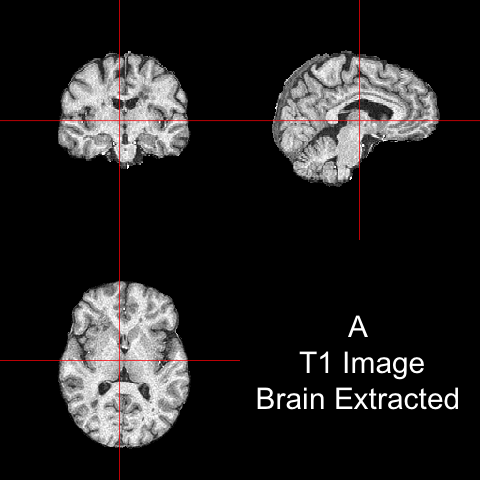
\includegraphics[width = 0.48\textwidth]{figure/Bet_Brain_A.png}
}
\hfill
  \subfloat{
  \label{bet_smooth}
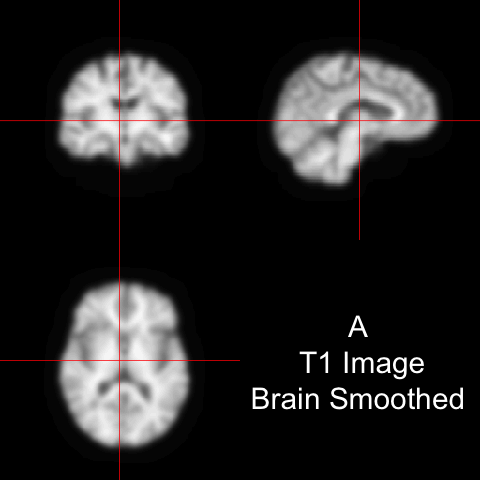
\includegraphics[width = 0.48\textwidth]{figure/T1_Smooth_Img.png}
}
\caption{{\bf Smoothing the Baseline T1 Brain Image.}  }
\label{fig:smooth}
\end{figure}


\section{Supplemental Material}

\subsection{Additional \pkg{fslr} Functionality}
Although the main goal of \pkg{fslr} is to interface R and FSL, there are a set of functions in \pkg{fslr} that are not designed to interface with FSL, but rather provide helper functions \code{nifti} objects form the \pkg{oro.nifti} package.  We will display 2 example functions: \code{cal\_img}, a function to reset the \code{cal\_min} and \code{cal\_max} slots on a \code{nifti} object, which are used to determine colors when plotting and \code{niftiarr}, which copies a \code{nifti} object and replaces the \code{.Data} slot with a provided array. 

Let us illustrate by discussing 2 ways to mask an image.  First we will read in the bias-corrected baseline T1 image and the brain mask from BET:


\begin{knitrout}
\definecolor{shadecolor}{rgb}{0.969, 0.969, 0.969}\color{fgcolor}\begin{kframe}
\begin{alltt}
\hlstd{base_t1} \hlkwb{=} \hlkwd{readNIfTI}\hlstd{(}\hlstr{"01-Baseline_T1_FSL_BiasCorrect"}\hlstd{,} \hlkwc{reorient}\hlstd{=}\hlnum{FALSE}\hlstd{)}
\hlstd{base_t1_mask} \hlkwb{=} \hlkwd{readNIfTI}\hlstd{(}\hlstr{"01-Baseline_T1_Brain_Mask"}\hlstd{,} \hlkwc{reorient}\hlstd{=}\hlnum{FALSE}\hlstd{)}
\end{alltt}
\end{kframe}
\end{knitrout}

One way to mask the T1 image is to multiply the image by the binary mask:
\begin{knitrout}
\definecolor{shadecolor}{rgb}{0.969, 0.969, 0.969}\color{fgcolor}\begin{kframe}
\begin{alltt}
\hlstd{base_t1_1} \hlkwb{=} \hlstd{base_t1} \hlopt{*} \hlstd{base_t1_mask}
\hlkwd{class}\hlstd{(base_t1_1)}
\end{alltt}
\begin{verbatim}
[1] "array"
\end{verbatim}
\end{kframe}
\end{knitrout}

We see that the resulting object is an array and not a \code{nifti} object. This may be a problem when trying to plot or manipulate this object using methods for \code{nifti} objects.  To address this problem, the \code{niftiarr} function in \pkg{fslr} inputs a \code{nifti} object and an \code{array}, and returns a \code{nifti} object with the provided \code{array} in the \code{.Data} slot, copying over the image information from the input \code{nifti} object.  

\begin{knitrout}
\definecolor{shadecolor}{rgb}{0.969, 0.969, 0.969}\color{fgcolor}\begin{kframe}
\begin{alltt}
\hlstd{base_t1_1} \hlkwb{=} \hlkwd{niftiarr}\hlstd{(base_t1, base_t1_1)}
\hlkwd{class}\hlstd{(base_t1_1)}
\end{alltt}
\begin{verbatim}
[1] "nifti"
attr(,"package")
[1] "oro.nifti"
\end{verbatim}
\end{kframe}
\end{knitrout}

Another way of masking the image is to subset the values of the image that are not in the mask and setting those values to $0$ (or some other value).
\begin{knitrout}
\definecolor{shadecolor}{rgb}{0.969, 0.969, 0.969}\color{fgcolor}\begin{kframe}
\begin{alltt}
\hlstd{base_t1_2} \hlkwb{=} \hlstd{base_t1}
\hlstd{base_t1_2[base_t1_mask} \hlopt{==} \hlnum{0}\hlstd{]} \hlkwb{=} \hlnum{0}
\hlkwd{class}\hlstd{(base_t1_2)}
\end{alltt}
\begin{verbatim}
[1] "nifti"
attr(,"package")
[1] "oro.nifti"
\end{verbatim}
\end{kframe}
\end{knitrout}

We see that this correctly returns an object of class \code{nifti}.  One problem is that the we have changed the data in the \code{nifti} object  \code{base\_t1\_2} but did not reset the other slots in this object to reflect this change.


In a \code{nifti} object, the \code{cal\_min} and \code{cal\_max} slots equal the minimum and maximum values, respectively, of the data.   The \code{orthographic} function (from \pkg{oro.nifti}) uses these values for plotting; also, if these slots do not equal the minimum and maximum, the \code{writeNIfTI} function (from \pkg{oro.nifti}) will fail.  The \code{cal\_img} is a simple helper function that will set the  \code{cal\_min} and \code{cal\_max} slots to the correct values.  Let us look at the range of the data and the \code{cal\_min} and \code{cal\_max} slots:
\begin{knitrout}
\definecolor{shadecolor}{rgb}{0.969, 0.969, 0.969}\color{fgcolor}\begin{kframe}
\begin{alltt}
\hlkwd{range}\hlstd{(base_t1_2)}
\end{alltt}
\begin{verbatim}
[1]   0.0000 409.3908
\end{verbatim}
\begin{alltt}
\hlkwd{c}\hlstd{(base_t1_2}\hlopt{@}\hlkwc{cal_min}\hlstd{, base_t1_2}\hlopt{@}\hlkwc{cal_max}\hlstd{)}
\end{alltt}
\begin{verbatim}
[1] 0 0
\end{verbatim}
\end{kframe}
\end{knitrout}
Note, one potential issue with \code{readNIfTI} function from \pkg{oro.nifti} is that the \code{cal\_min} and \code{cal\_max} slots were both read as zero.  Let us set these to the range using the \code{cal\_img} command from \pkg{fslr}:
\begin{knitrout}
\definecolor{shadecolor}{rgb}{0.969, 0.969, 0.969}\color{fgcolor}\begin{kframe}
\begin{alltt}
\hlstd{base_t1_2} \hlkwb{=} \hlkwd{cal_img}\hlstd{(base_t1_2)}
\hlkwd{range}\hlstd{(base_t1_2)}
\end{alltt}
\begin{verbatim}
[1]   0.0000 409.3908
\end{verbatim}
\end{kframe}
\end{knitrout}
We see that after these operations are done 2 in different ways, the resulting \code{nifti} objects are equivalent.  
\begin{knitrout}
\definecolor{shadecolor}{rgb}{0.969, 0.969, 0.969}\color{fgcolor}\begin{kframe}
\begin{alltt}
\hlkwd{all.equal}\hlstd{(base_t1_1, base_t1_2)}
\end{alltt}
\begin{verbatim}
[1] TRUE
\end{verbatim}
\end{kframe}
\end{knitrout}

Additional helper functions such as these are included in \pkg{fslr} for plotting and image manipulation.

%\section{Difference between Images}
%Now that we have the images in the same space and a mask for the brain image, we can take a difference of brain-only tissues.  







%
%\begin{figure}
%  \subfloat{
%  \label{diff_img}
%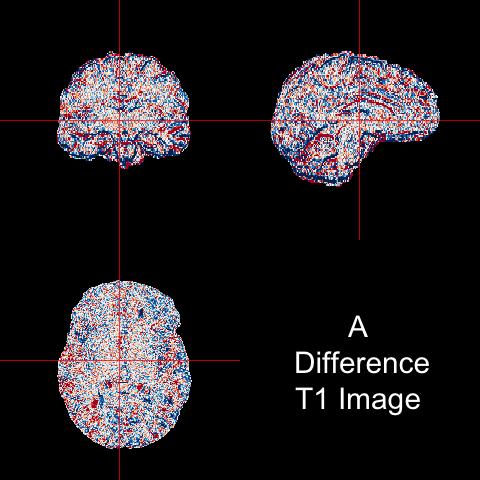
\includegraphics[width = 0.31\textwidth]{figure/T1_Diff_Img_Col.png}
%}
%\hfill
%  \subfloat{
%  \label{diff_hist}
%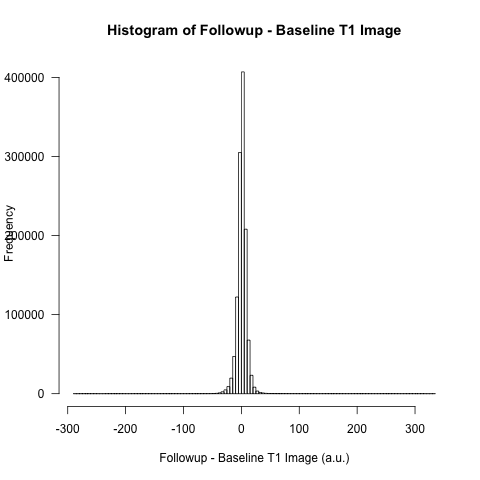
\includegraphics[width = 0.31\textwidth]{figure/T1_Diff_Hist.png} 
%}
%\hfill
%  \subfloat{
%  \label{diff_plot}
%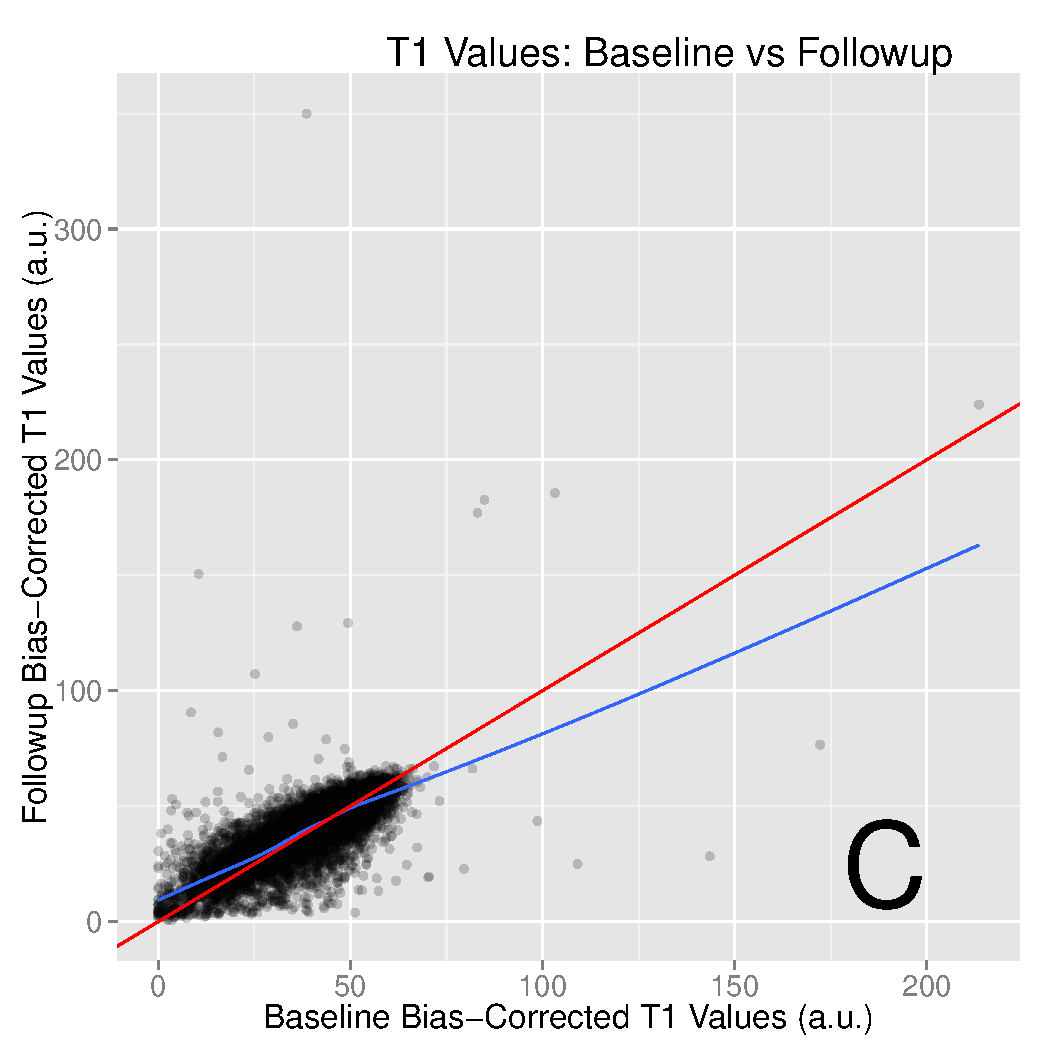
\includegraphics[width = 0.31\textwidth]{figure/plot_base_follow_data.pdf} 
%}
%\caption{{\bf Differences from Baseline to Followup T1 Image.}  In~\protect\subref{diff_img}, we show the difference image, subtracting the followup bias-corrected T1 image from the baseline bias-corrected T1 image, where colors in blue represent negative values (baseline is higher) and red represents positive values (baseline is lower).  The histogram of these differences, for values within the brain mask are presented in~\protect\subref{diff_hist} and the scatterplot comparing these two images is presented in~\protect\subref*{diff_plot}, where red line represents the 45$^{\circ}$ diagonal line and the blue represents a LOESS smoother.}
%\label{fig:diff}
%\end{figure}
%
%
%\subsection{Smoothing Difference Images}
%We can smooth the difference image using a Gaussian kernel ($\sigma = 3$mm) to 
%locally average the differences between the images (Figure~\ref{fig:diff_smooth}\protect\subref*{diff_img_smooth}).  If we color the image by deciles (Figure~\ref{fig:diff_smooth}\protect\subref*{diff_img_csmooth}), we can note a pattern across the image.  MRI images acquired have arbirtrary units, it is hard to compare the raw intensities across days, however.  We would need to do an intensity-based normalization for comparison, such as the White Stripe method \citep{whitestripe} or use a procedure that accounts for this, such as a modeling framework.  As this is not the focus of this demonstration of software, we will not discuss methods for achieving this.  













%\begin{enumerate}
%\item Porting similar to nipype
%\item Open source and readily available
%\item Allows users who know R to leverage that knowledge
%\item R in and R output
%\item Already made suite of tools - not re-inventing the wheel.
%\end{enumerate}


\address{John Muschelli\\
  PhD Student\\
  Johns Hopkins Bloomberg School of Public Health, \\
  Baltimore, MD 21231 \\
  USA
  }
\email{jmuschel@jhsph.edu}

\address{Elizabeth Sweeney\\
  PhD Student\\
  Johns Hopkins Bloomberg School of Public Health\\
  Baltimore, MD 21231 \\
  USA \\
  Special Volunteer 
  Translational Neuroradiology Unit, Neuroimmunology Branch, National Institute of Neurological Disease and Stroke, National Institute of Health \\
  Bethesda, MD 20892\\
  USA
  }
\email{emsweene@jhsph.edu}

\address{Martin Lindquist\\
  Associate Professor\\
  Johns Hopkins Bloomberg School of Public Health, \\
  Baltimore, MD 21231 \\
  USA
  }
\email{mlindqui@jhsph.edu}

\address{Ciprian Crainiceanu\\
  Professor\\
  Johns Hopkins Bloomberg School of Public Health, \\
  Baltimore, MD 21231 \\
  USA
  }
\email{ccrainic@jhsph.edu}

\bibliography{FSLR}
%\AtEveryBibitem{\clearfield{note}}    % clears notes

%
%\section{Supplemental Material}
%\section{Z-score and threshold}








